\section{Introduction}

Vision-language-action (VLA) models achieve high task success on manipulation benchmarks~\cite{brohan2023rt2, kim2024openvla, kim2025oft}, but behavioral safety does not follow. On SafeLIBERO Level~I~\cite{hu2025vlsa}, OpenVLA-7B reaches 87.8\% Task Success Rate but only 74.5\% Collision Avoidance Rate (CAR), with per-task collision rates reaching 43--93\% on the three most constrained tasks (Appendix, Table~\ref{tab:per_task}).

Two active research threads address related but distinct aspects. The first enriches VLAs with auxiliary spatial prediction (occupancy grids, depth maps, point clouds)~\cite{li2026spatialforcing, yuan2025depthvla, wu2025spatialvla, liu2025occvla}. At least fifteen such methods have appeared in the past year~\cite{wu2026stvla, chen2026gstvla, tu2026sgvla, xiao2026stemvla, li2025pointvla, sun2025geovla, bhat20253dcavla, li2025qdepthvla, abouzeid2025geoaware, rao2026augvla3d, li2026corridorvla}, all reporting improved task success under the implicit assumption that spatial awareness yields safer behavior. The second targets VLA safety directly through runtime action filtering~\cite{hu2025vlsa, zhai2026cofreevla, raja2024ogmcbf} or constrained RL~\cite{zhang2025safevla}. These lines are disconnected: no spatial method evaluates collision avoidance, and no safety method examines spatial representations. A recent survey~\cite{li2026vlasafety} confirms this gap. Moreover, single-factor ablations, the dominant methodology, cannot decompose joint effects of multiple design choices; only a factorial design can determine whether factors like gradient flow and normalization type interact or combine independently.

\begin{figure*}[t]
\centering
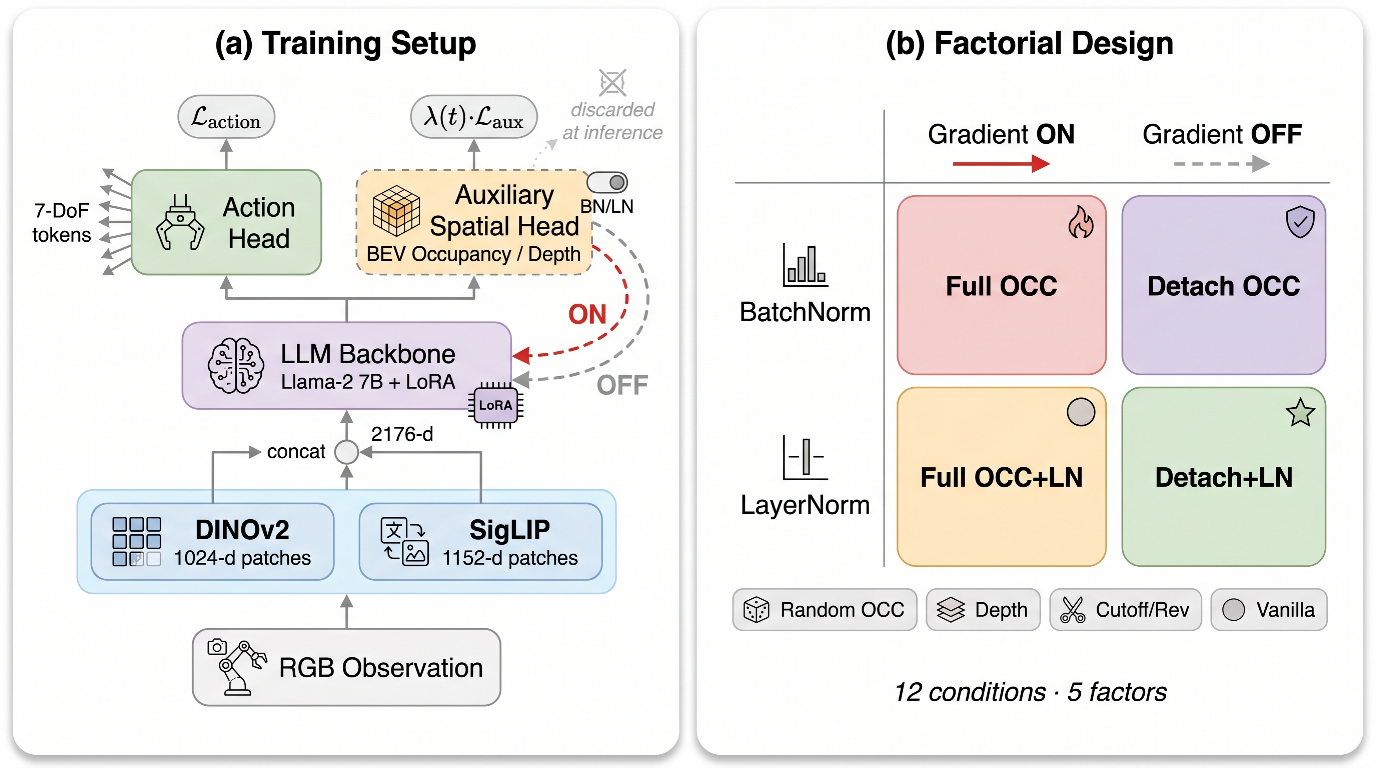
\includegraphics[width=\textwidth]{figures/fig1_architecture_pb.pdf}
\caption{\textbf{Training setup and factorial design.} \textbf{(a)}~OpenVLA-7B with dual vision encoders (DINOv2 + SigLIP) and an auxiliary spatial head (bird's-eye view occupancy or depth), discarded at inference. \textbf{(b)}~$2{\times}2$ factorial crossing gradient flow (ON/OFF) and normalization (BN/LN), plus Vanilla baseline and 7 single-factor ablations probing label content, reference frame, and temporal extent.}
\label{fig:overview}
\end{figure*}

% fig:results_bar moved into fig:car_factorial (a)

We ask a direct question: does auxiliary spatial supervision during VLA fine-tuning improve collision avoidance? We conduct a systematic factorial study using OpenVLA-7B~\cite{kim2024openvla} with LoRA~\cite{hu2022lora}. A core $2{\times}2$ factorial crosses gradient flow (ON/OFF) with normalization (BN/LN); seven additional single-factor ablations probe label content, spatial reference frame, and temporal extent, twelve conditions in total (Figure~\ref{fig:overview}). The factorial design can detect interactions that single-factor studies miss; here, it establishes that the two main effects are additive (\S\ref{sec:results}), a practically important finding that prior work could not have obtained.

The central finding is that \textbf{Detach+LN consistently outperforms Vanilla}, raising CAR from $0.745$ to $0.802$ with a large effect size. The factorial design reveals why: gradient flow through BatchNorm degrades safety, while LayerNorm provides a consistent advantage, and these two effects combine additively. Only the BN + gradient flow combination falls below Vanilla. Spatial label content showed no detectable effect under the v1 codebase (\S\ref{sec:results}).

Our contributions:
\begin{enumerate}[nosep,leftmargin=*]
    \item \textbf{Two additive factors govern safety, not spatial content.} Detached gradients with LayerNorm yield the highest collision avoidance rate, reliably outperforming the no-auxiliary baseline with a large effect size. A $2{\times}2$ factorial identifies two additive factors: gradient flow through BatchNorm degrades safety; LayerNorm provides a consistent protective effect. These safety effects are invisible to standard task-success benchmarks (TSR ANOVA all $p{>}0.27$), explaining why fifteen prior methods did not detect them. Spatial label content shows no detectable influence under the original codebase (Table~\ref{tab:main_results}, Figure~\ref{fig:car_factorial}b), with the normalization advantage amplifying fourfold on physically constrained tasks where safety margins are thinnest.

    \item \textbf{Factorial methodology for VLA auxiliary heads.} The first systematic factorial comparison of how auxiliary head design choices combine during VLA fine-tuning. The factorial design establishes that effects are additive, a conclusion single-factor ablations cannot reach (\S\ref{sec:ablation}, Table~\ref{tab:ablation_design}).

    \item \textbf{Actionable guidelines at zero cost.} Do not add auxiliary spatial heads with gradient flow under BN. If required, use detached gradients with LayerNorm. BN + gradient flow additionally exhibits $5$--$7{\times}$ cross-seed variance, making safety outcomes unpredictable across training runs. No ground-truth spatial labels are needed; the auxiliary head is discarded at inference (\S\ref{sec:discussion}).

    \item \textbf{Codebase sensitivity as a confound.} Implementation details dominate safety signals: a single code revision shifts CAR by up to 8.6\,pp, exceeding the largest experimental effect (${\leq}5.7$\,pp), questioning the reproducibility of safety claims across existing spatial VLA methods (\S\ref{sec:discussion}, Appendix~\ref{app:codebase}).
\end{enumerate}